\documentclass{anstrans}
%%%%%%%%%%%%%%%%%%%%%%%%%%%%%%%%%%%
\title{Online Processing System for Molten Salt Reactors}
\author{David Barnett, Nathan Glaser, and Joseph F. Specht IV}

\institute{
Department of Nuclear, Plasma, and Radiological Engineering, University of Illinois Urbana-Champaign \\ davidbb2@illinois.edu, nglaser3@illinois.edu, jspecht3@illinois.edu}

% Optional disclaimer: remove this command to hide
%\disclaimer{Notice: this manuscript is a work of fiction. Any resemblance to actual articles, living or dead, is purely coincidental.}

%%%% packages and definitions (optional)
\usepackage{graphicx} % allows inclusion of graphics
\usepackage{booktabs} % nice rules (thick lines) for tables
\usepackage{array}
\usepackage{microtype} % improves typography for PDF
\usepackage{multicol}
\usepackage{enumerate}

\newcommand{\SN}{S$_N$}
\renewcommand{\vec}[1]{\bm{#1}} %vector is bold italic
\newcommand{\vd}{\bm{\cdot}} % slightly bold vector dot
\newcommand{\grad}{\vec{\nabla}} % gradient
\newcommand{\ud}{\mathop{}\!\mathrm{d}} % upright derivative symbol
\newcommand{\iso}[2]{$^{#2}$#1}
\begin{document}
%%%%%%%%%%%%%%%%%%%%%%%%%%%%%%%%%%%%%%%%%%%%%%%%%%%%%%%%%%%%%%%%%%%%%%%%%%%%%%%%
\section{Introduction}
The Department of Energy predicts domestic electricity demand could more than double by 2050. However, achieving net-zero carbon energy production would require roughly an addition of 700 to 900 GigaWatts of clean generation capacity \cite{doe-summary}. For reference, the current generation capacity of the United States is 1300 GW \cite{gen-cap}. As the energy demands surge over the next 30 years, advanced nuclear reactors will be instrumental in supplanting fossil fuels and creating a net-zero carbon future.

According to the 2018 R\&D outlook published by the Gen IV International Forum (GIF), there are six promising Generation IV reactor designs: (i) sodium-cooled fast reactors (SFRs), (ii) very high temperature reactors (VHTRs), (iii) gas-cooled fast reactors (GFRs), (iv) molten salt reactors (MSRs), (v) lead-cooled fast reactors (LFRs), and (vi) supercritical water-cooled reactors (SCWRs). Of these advanced reactors, MSRs are of particular interest for their high thermal efficiency, breeding capabilities, and versatile fuel types.

One of the important R\&D challenges laid out by the GIF is on-site fuel processing \cite{GIF2018Roadmap}. MSRs are particularly well suited for on-site fuel processing due to their circulating, liquid fuel. In this paper, we discuss removal methods for tritium, neutron poisons, and protactinium from the primary loop of thorium-uranium (Th-U) fueled MSRs. Removing tritium is crucial for the lifetime of the reactor as tritium at high temperatures, like those in MSRs, is highly corrosive threatening the integrity of structural materials \cite{tritium-damage}. The removal of relevant neutron poisons, like \iso{Xe}{135}, is crucial to an improved neutron economy, and allows reactors to perform load-following. Finally, in T-U fueled MSRs, $^{233}Pa$ is born from $^{232}Th(n,\gamma)$ and decays into $^{233}U$ with a half-life of 26.975 days. $^{233}Pa$ is a parasitic absorber however, therefor it must be allowed to decay into $^{233}U$ free from bombarding neutrons, otherwise the breeding reaction will be for naught. 

To address this demand for on-site fuel processing, we propose a modular online processing system. This system will be placed after an MSR's heat exchanger on the primary loop, and contains three main removal mechanisms: helium gas sparger, graphene absorption columns, and electrochemical ports. Each of these methods, as well as how they are coupled together, will be discussed in more detail in the consequent sections.

%%%%%%%%%%%%%%%%%%%%%%%%%%%%%%%%%%%%%%%%%%%%%%%%%%%%%%%%%%%%%%%%%%%%%%%%%%%%%%%%
\section{Theory}
Before explaining the proposed online-processing systems, the theory detailing the standard operation of MSRs is presented, aswell as the isotopes we aim to remove with a justification for each. Finally, this section ends with a discussion of MSR design limitations.

\subsection{Comparison of Online and Offline Processing}
Traditionally, most MSRs use offline processing systems for contaminant removal in the fuel salt \cite{msbrreprocessing}. However, MSRs utilizing the Th-U fuel notably siphon $^{233}$Pa from the fuel salt online. Aside from $^{233}$Pa siphoning, MSR fuel salt processing is performed offline and batch-wise -- the fuel-salt is (i) diverted from the reactor, (ii) treated with the appropriate processing system, (iii) re-united with the main fuel-salt line, and (iv) pumped back into the reactor core \cite{msbrreprocessing}.

By necessity, offline reprocessing diverts a fraction of the fuel-salt from the main fuel-salt \cite{XeRemoval}. The diverted fuel-salt is apportioned into batches and operated on in isolation. Each batch may remain isolated for multiple days. For example, $^{135}$Xe is removed for 47 hours, enough time for 97\% of the $^{135}$Xe to decay \cite{diversion}.

Although most removal efficiencies are high, isolating the fuel-salt for an extended period has two major draw-backs of interest. The first drawback is the increase in required fuel-salt inventory. Every batch outside of the reactor is required for offline processing and cannot contribute to nuclear fission. Second, MSRs using offline processing are unable to load follow. As the neutron poisons are removed ex-core, the in-core $^{135}$Xe concentration is unaffected by the batch-wise processing. However, if an MSR used online processing, these issues would be diminished.

Like offline processing, MSRs using online processing may divert a portion of the fuel-salt to a secondary loop. However, the secondary loop would contain the fuel-salt for minutes compared to days in offline systems. In online processing, fuel-salt contaminants are removed in potentially lower efficiencies, but continually. The continuous removal of contaminants allows MSRs to have lower equilibrium concentrations than offline processing.

\subsection{Isotopes of Concern}
For this report, we considered the removal of $^{135}$Xe, T, and $^{133}$ Pa for various reasons. First, $^{135}$Xe is a strong neutron poison. As such, the continued elimination of $^{135}$Xe results in a positive reactivity insertion and a more economic reactor. Second, T is highly permeable in metals a high temperatures, like those in MSRs. The permeation of T into metals causes embrittlement and swelling once the T decays into $^3$He. Therefore, removing T would theoretically extend the lifetime of metal components. Finally, $^{233}$Pa is a transmute of $^{232}$Th and decays into $^{233}$U with a half life of roughly 27 days. However, $^{233}$Pa can transmute into $^{234}$U, a parasitic neutron absorber. By isolating $^{233}$Pa, we would improve the breeding ratio of the MSR by reducing parasitic absorption.

\subsection{Hastelloy and Antimony}. The pipe lining most commonly proposed for use in Molten salt reactors of both Fluoride and Chlorine salts it Hastelloy, Particularly Hastelloy-N. Hastelloy is a a nickel-based alloy, and as such, it's primary corrosion method is inter-granular corrosion caused by tellurium attack phenomena. This corrosion is sited as the limiting factor for the upper temperature limits in molten salt reactors, as increased heat speeds this type of corrosion. Tellurium is present in most molten salt reactors through the decay of antimony; a fission product. If antimony was either not generated, or removed at the time of generation, it would be possible to raise the safe operating temperature of molten salt reactors from the current 704C to a possible maximum of 871C \cite{NRCHastelloy}, but no known method of tellurium removal has been proposed that would safely allow such an increase, and any such method would by design have some degree of risk during failure. As such, in locations of Hastelloy use in the proposed design, a temperature limit of 704C will have to be observed, but represents a possible location of future improvement with either a different pipe lining, or breakthroughs in tellurium removal.
\subsection{Flow Rate}

Flow rate is a crucial parameter for MSRs. Higher flow rates dictate lower Delayed Neutron Precursor (DNP) concentrations in the core, and also lower chance for temperature build-up in the core. This results in less operator control over the reactor, and worse thermal efficiency, respectively. Alternatively, too low of flow can result in poor heat transfer. 

% Pe

\section{Removal Systems}\label{remsys}
As previously mentioned, our proposed system leverages three existing technologies, however each have been adapted to work within our Modular On-line Processing System (MOPS). To refresh, these systems are: helium gas spargers, parallel graphene absorption columns, and electrochemical ports.

\subsection{Removal Sub-Processes}
\textbf{Helium Gas Spargers} are traditionally proposed as an off-line bulk processing system for molten fuel-salt. They typically work by injecting helium gas into the bottom of a fuel-salt filled tank, allowing the bubbles to flow up through the fuel-salt and pulling out gasses not in solution (noble gasses, some phases of tritium). This process is driven by diffusion, where the gasses in the fuel-salt diffuse to the helium bubbles. This process, because it is diffusion driven, takes an appreciable amount of time to process large quantities of salt \cite{XeRemoval}. To address this demand we will have a large number of spargers along our system, each with a greatly reduced volume of fuel-salt to process than traditional proposals. To ensure adequate time for appreciable diffusion to occur, our system temporarily diverges the fuel-salt flow, allowing for much slower linear-velocities. To ensure we have adequate flow speeds through the core, our system converges the flow again. 

To minimize the gas content of the fuel-salt prior to it's pass through the pump, and consequently the core, we utilize two gas separation techniques. The first is an internal gas blanket and the second is a dedicated gas separator. The internal gas blanket is a region of gas above the fuel-salt within our MOPS, that serves as a destination for bubbles that make it through the fuel-salt. These bubbles are then siphoned off through pressure valves. The dedicated gas separator is placed after the flow convergence phase, and immediately prior to the pump. This separator removes all of the residual gas bubbles that did not make it through the fuel-salt to the blanket.\newline

\textbf{Parallel Graphene Absorption Columns} are blocks of graphene that are parallel to the flow. These blocks act as a diffusive destination for tritium, noble gasses, and noble metals. This is because graphene has a very high specific surface area, which enables strong diffusive forces. The reason these blocks are not used as traditional filters where the flow would flow through them and are instead placed parallel to the flow, is because the graphene is mostly impermeable to the UF$_4$-FLiBe --- despite being a porous media. In our system, we use this to our advantage. The parallel graphene absorption columns will be placed such that they form channels, acting as barriers and restricting cross-flow. These discrete channels enable channel-tailored operation with the adaptive processing modules (one channel preferentially removes one nuclide, and another removes another).  \newline

\textbf{Adaptive Processing Modules}. By creating a modular pipe structure that splits into multiple channels, an electrode network could be created that would allow most pyroprocessing methods used for lanthanide and actinide separations to be directly implemented within the system. By using soluble metal solvents such as aluminum or an aluminum-copper alloy, A solid precipitation is created on the inserted electrode \cite{NRCPyro}, and by controlling the electro-potential difference between the fluid and the electrode, specific elements can be preferentially removed if desired. Small scale applications of similar offline techniques have already been done by the French Commissariat à l’Energie Atomique, with the only major change proposed being an online application of the technique using a combination of slowed flow and some form of agitator to speed up diffusion of removable materials in the liquid fuel. This would circumvent the negatives of the generally used methods of concurrent extraction and siphoning, and potentially allow for the Helium Gas Spargers to be used as agitators for the system. The major downsides of this system would be the complex nature of electrochemical systems elongating the primary fuel loop, and the need for reactor-specific solutions and set ups preventing repeatability, and not easily lending itself to mass production.

\subsection{Modular On-Line Processing System}\label{omps}
To begin the presentation of our proposed system, we first present an overview of the primary loop. 

\begin{figure}[!h]
    \centering
    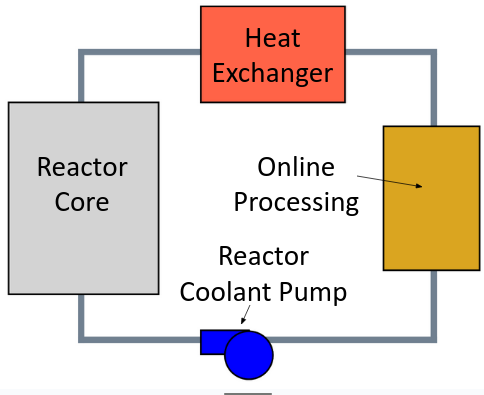
\includegraphics[width=0.5\linewidth]{pictures/system.png}
    \caption{Primary loop of molten salt reactor utilizing the MOPS}
    \label{fig:enter-label}
\end{figure}

The MOPS would be installed antecedent to the reactor coolant pump and subsequent to the heat exchanger. 

The MOPS diverges the flow, greatly increasing the total cross-sectional area of the pipe and effectively reducing the linear velocity through each channel. This increased cross-sectional area is then divided into multiple sub-channels, each divided by a parallel graphene absorption column. Although the final dimensions of the MOPS, as well as the number of channels, are currently undergoing optimization, a mock-up of the MOPS is presented below in Figures \ref{fig:xs} and \ref{fig:topdown}. For scale, the diameter of the incoming pipe (from the heat exchanger) will be much smaller than the width of a channel. The UF$_4$FLiBe salt is in green, and the gas blanket is the white block above the FLiBe. Each of the blue and red cylinders are an adaptive processing module, and each of the upwards-facing gray triangles (and gray circles) are the helium gas spargers. Finally the black rectangles forming the channels are the parallel graphene absorber columns. Notably, the helium gas spargers were omitted from the 4 right most channels in Figure \ref{fig:topdown} for simplicity, as they are there just under the adaptive processing modules. These spargers are strategically placed under the modules to induce turbulent flow around the modules, enabling mixing effects to occur. This is done to increase the efficiency of the modules, as mixing is a crucial step in electrochemical processes. 

\begin{figure}[!h]
    \centering
    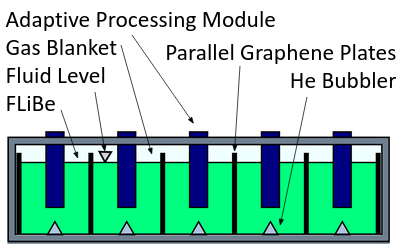
\includegraphics[width=1.\linewidth]{pictures/xs.png}
    \caption{Cross-sectional (xz) cut-through of the MOPS}
    \label{fig:xs}
\end{figure}

\begin{figure}[!h]
    \centering
    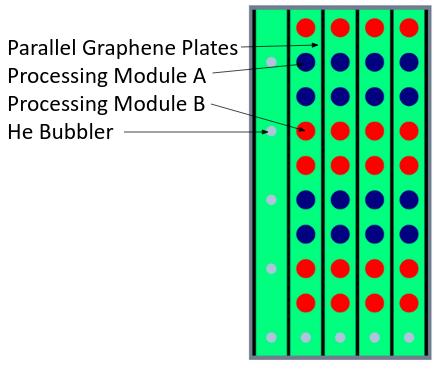
\includegraphics[width=1.\linewidth]{pictures/topdown.png}
    \caption{Top-down (xy) cut through of the MOPS}
    \label{fig:topdown}
\end{figure}

\subsection{Modular On-Line Processing System Implications}\label{ompsI}
There are strong implications of employing the MOPS on the overall reactor system. The most impactful are neutron poison removal, reduced flow-speeds, and a greater pressure drop from the core outlet to the reactor coolant pump. Neutron poison removal enables load-following maneuvers with the reactor, effectively matching the reactor output to the energy-grid demand. Reduced flow speeds in the core result in more operator control over the reactor and also higher temperatures in the core. The greater operator control stems from an increased quantity of Delayed Neutron Precursors (DNPs) decaying in the core as opposed to the piping, resulting in a greater $\beta_{eff}$. Further, the higher temperatures actually enable greater Carnot efficiency, as this efficiency is defined as 1 - $\frac{T_c}{T_h}$, and so a greater difference between the two yields a greater thermal efficiency. Finally, a greater pressure drop from the core to the reactor coolant pump increases the load on the pump, which may necessitate an additional pump. 

%%%%%%%%%%%%%%%%%%%%%%%%%%%%%%%%%%%%%%%%%%%%%%%%%%%%%%%%%%%%%%%%%%%%%%%%%%%%%%%%

\section{Methods}
\subsection{Nuclide Source Rates}
To determine nuclide source rates, we are utilizing a simplified MSBR \cite{msbrreprocessing} model in OpenMC \cite{OpenMC}. This model is a cylinder with the real reactor height, and a radius set to enforce the volume of the cylinder to be equal to that of the effective fuel volume in the MSBR. This model utilizes the detailed UF$_4$FLiBe concentrations and enrichment as the only material. To obtain steady state per-pass production rates for nuclides, the $^{233}U$ concentration was artificially increased until $k_{eff}$ reached roughly 1. Then, to obtain the per-pass source rates as a function of fuel residency in the core, we ran a depletion solve with 20 time steps, each separated by 15 seconds for an end time of 5 minutes. We assumed fuel moved batchwise through the core for this initial model and recognize the limitations this imposes.

\subsection{Unresolved Methods}
This work is still ongoing, and thus we have not finalized the models we will use for verification and validation. Potential plans for future work involves utilizing Cardinal \cite{cardinal} to model the pressure drop across the MOPS, as-well as to determine the efficacy of our proposed work with high-fidelity thermal hydraulic and neutronic analysis, enforcing our equilibrium concentrations unto the fuel-salt in the (higher fidelity) MSBR model.

\section{Results}
This work is still ongoing, however we have preliminary results for the nuclide source rates as a function of in-core residency. 
\begin{figure}[!h]
    \centering
    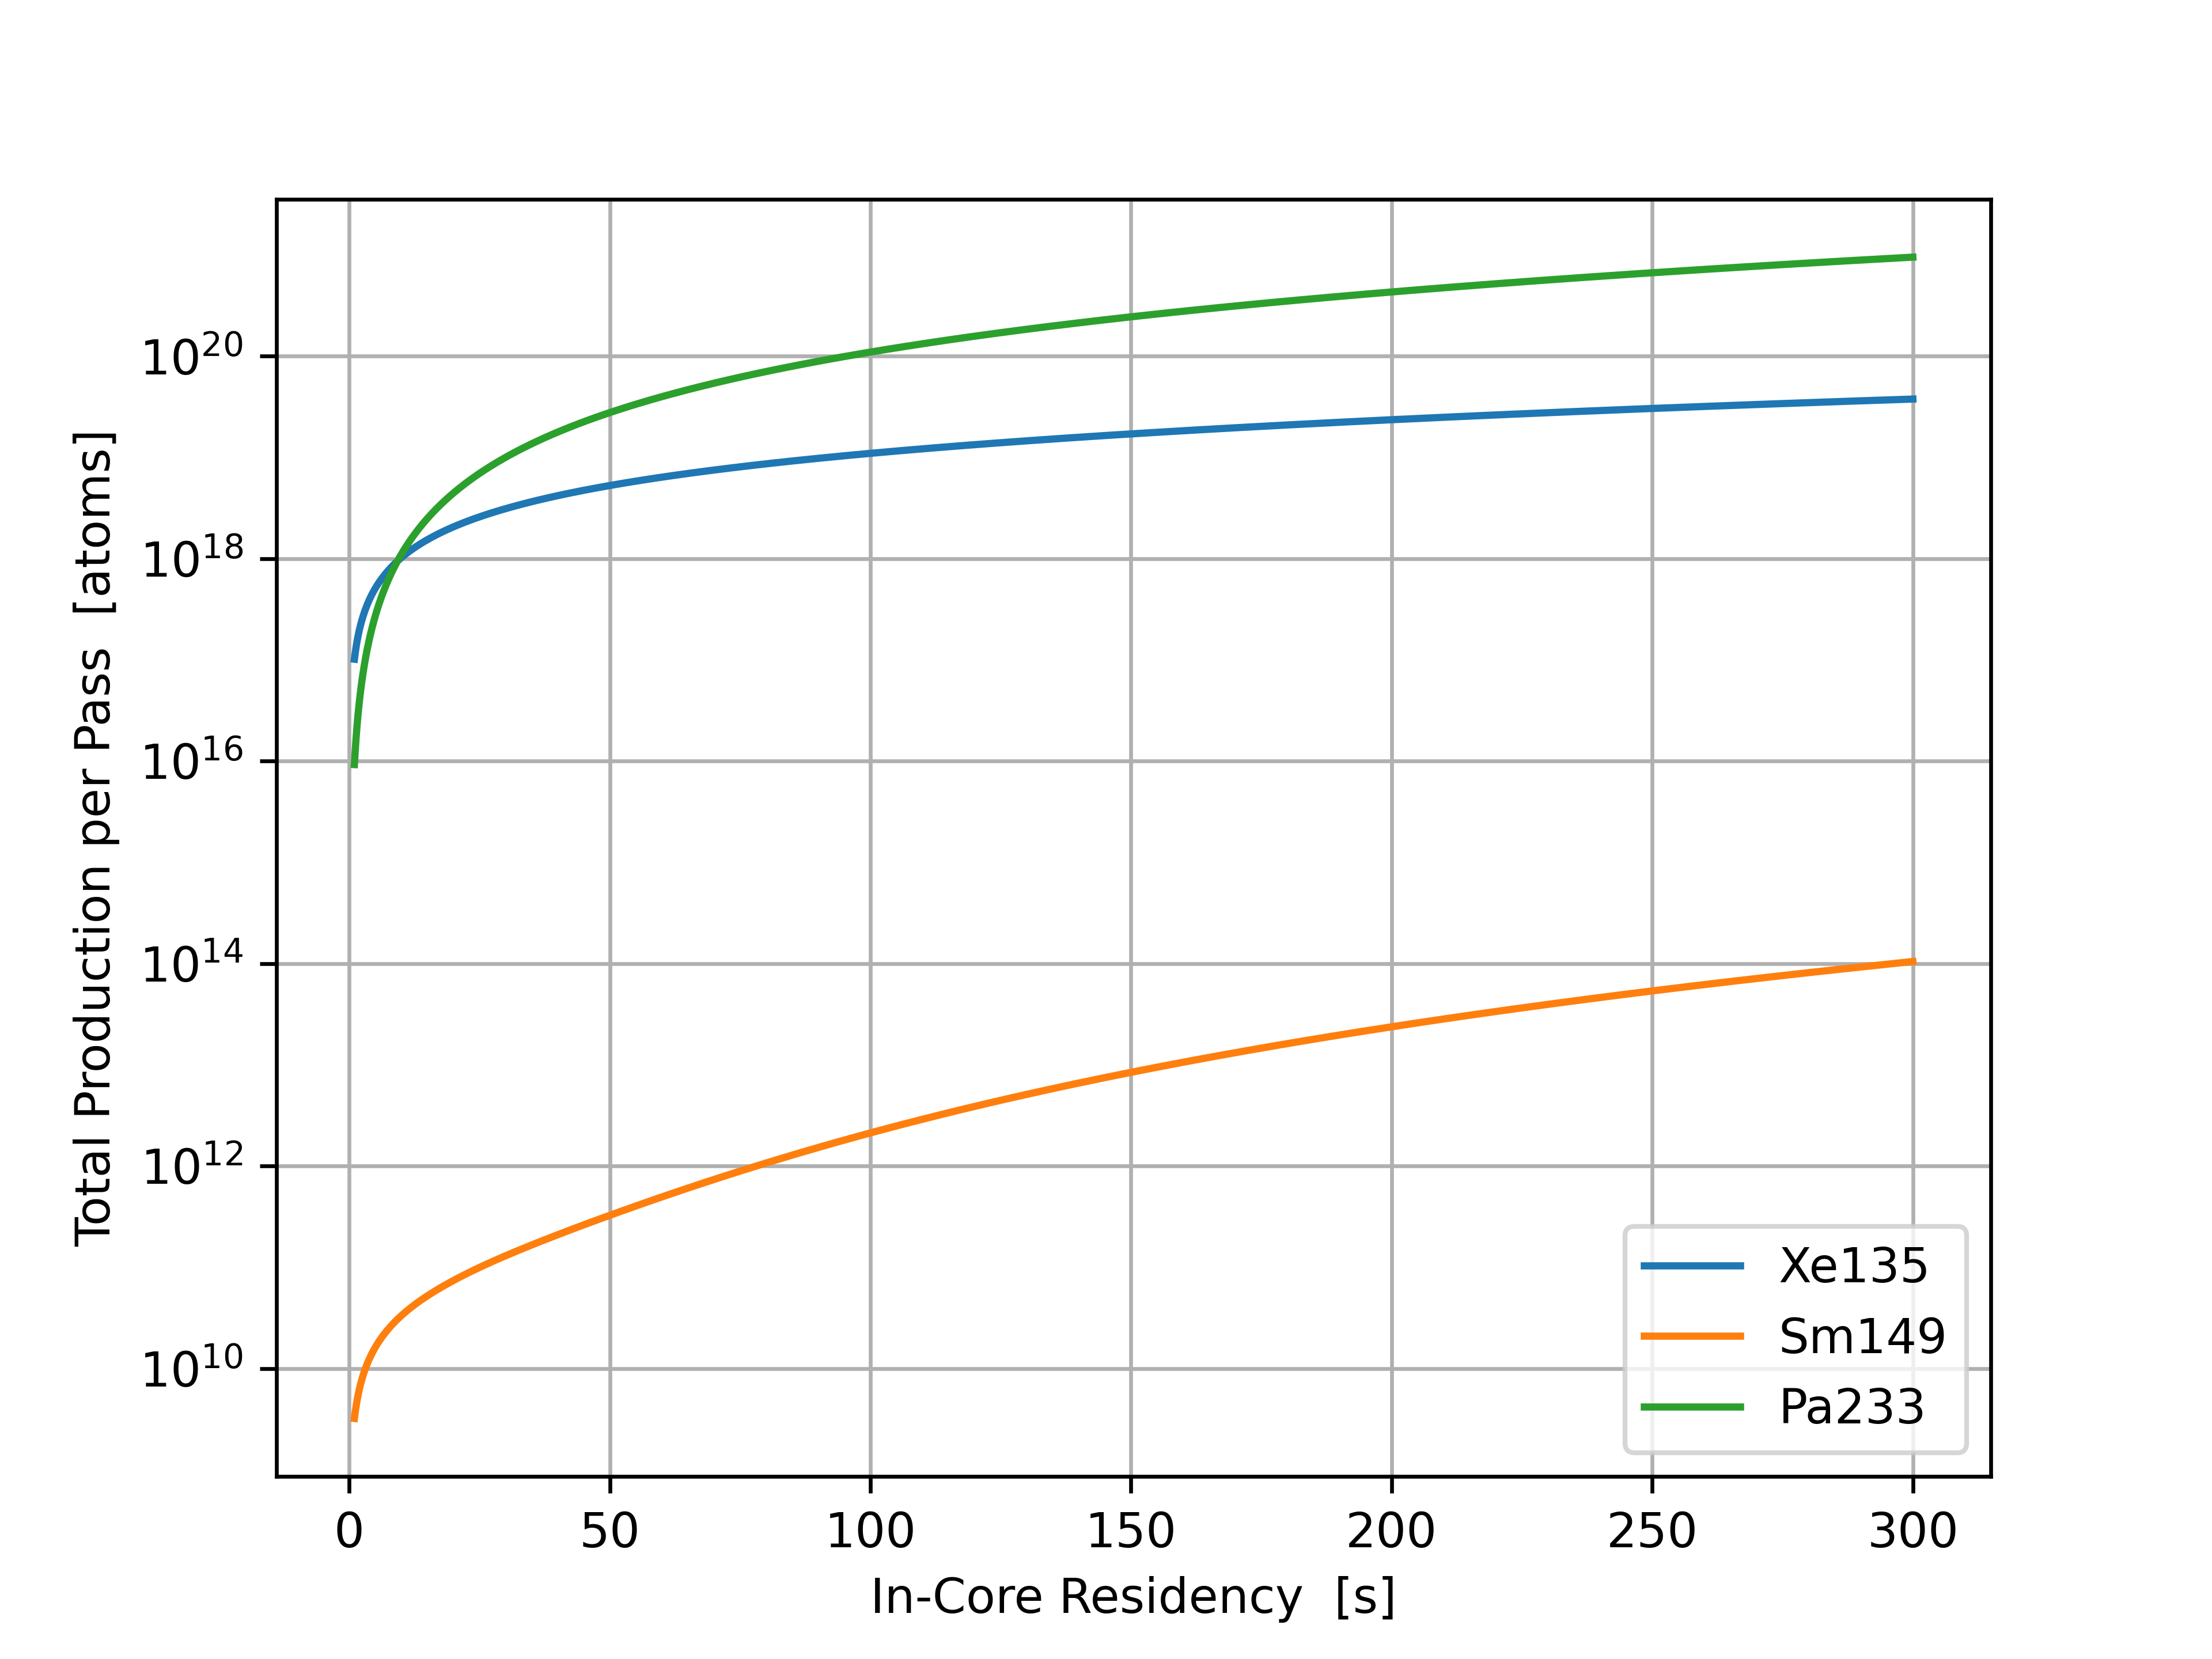
\includegraphics[width=1.\linewidth]{pictures/sourceplot.png}
    \caption{Per pass source rates as a function of in-core residency}
    \label{fig:source}
\end{figure}

Ideally, when determining the efficiencies of our systems, we would like to have sufficient nuclide concentration for our system to fiscally make sense to operate, and so we will be investigating the higher bounds for the in-core residency. Further this higher residency implies slower flow, ideal for improved efficiency for our system.

Much of this work is still under-going and so this concludes our preliminary results.

%%%%%%%%%%%%%%%%%%%%%%%%%%%%%%%%%%%%%%%%%%%%%%%%%%%%%%%%%%%%%%%%%%%%%%%%%%%%%%%%

\section{Conclusions}
We propose a novel modular online processing system, MOPS, which enables load-following maneuvers for molten salt reactors, as well as greatly improved fuel utilization. Further, our proposed system requires reduced pump speeds (compared to the MSBR and MSRE \cite{MSRE}) which greatly increase operator control over the reactor, aswell as the carnot efficiency of the reactor. We have determined the per-pass source rates of relevant nuclides as a function of fuel-salt in-core residency, and aim to determine optimal design parameters to reach desired removal efficiencies and nuclide concentrations. With this finished model, we aim to perform high-fidelity neutronics and thermal-hydraulics modeling with Cardinal to validate the efficacy of our design with respect to standard reactor operation. 

%%%%%%%%%%%%%%%%%%%%%%%%%%%%%%%%%%%%%%%%%%%%%%%%%%%%%%%%%%%%%%%%%%%%%%%%%%%%%%%%

\bibliographystyle{ans}
\bibliography{bibliography}
\end{document}

